\documentclass{scrreprt}
\usepackage{graphicx}
\usepackage{listings}
\usepackage{underscore}
\usepackage[bookmarks=true]{hyperref}
\usepackage[utf8]{inputenc}
\usepackage[english]{babel}
\usepackage{subfigure}
\usepackage{hyperref}
\usepackage[table,xcdraw]{xcolor}
\setlength{\footskip}{140pt}
\graphicspath{ {images/} } 
\hypersetup{
    bookmarks=false,    % show bookmarks bar?
    pdftitle={Software Requirement Specification},    % title
    pdfauthor={Matthew Berger},                     % author
    pdfsubject={TeX and LaTeX},                        % subject of the document
    pdfkeywords={TeX, LaTeX, graphics, images}, % list of keywords
    colorlinks=true,       % false: boxed links; true: colored links
    linkcolor=blue,       % color of internal links
    citecolor=black,       % color of links to bibliography
    filecolor=black,        % color of file links
    urlcolor=purple,        % color of external links
    linktoc=page            % only page is linked
}%
\def\myversion{1.0 }
\date{}
%\title
\usepackage{xcolor,colortbl}
\newcommand{\mc}[2]{\multicolumn{#1}{c}{#2}}
\definecolor{LightGray}{gray}{0.95}
\definecolor{Gray}{gray}{0.85}
\definecolor{LightCyan}{rgb}{0.88,1,1}

\newcolumntype{a}{>{\columncolor{Gray}}p{0.3\linewidth}}
\newcolumntype{b}{>{\columncolor{white}}p{0.7\linewidth}}
\newcolumntype{d}{>{\columncolor{LightGray}}p{0.3\linewidth}}
\newcolumntype{e}{>{\columncolor{white}}p{0.6\linewidth}}
\newcolumntype{f}{>{\columncolor{LightGray}}p{0.2\linewidth}}
\newcolumntype{g}{>{\columncolor{Gray}}p{0.2\linewidth}}
\newcolumntype{h}{>{\columncolor{white}}p{0.8\linewidth}}

\begin{document}

\begin{flushright}
    \rule{16cm}{5pt}\vskip1cm
    \begin{bfseries}
        \Huge{SOFTWARE REQUIREMENTS\\ SPECIFICATION}\\
        \vspace{1.6cm}
        for\\
        \vspace{1.6cm}
        $NAVATAR$\\
        \vspace{1.6cm}
        \LARGE{Version \myversion approved}\\
        \vspace{1.6cm}
        Prepared by Matthew Berger, Liam Gomez, and Connor Parkinson\\ 
        \vspace{1.6cm}
        Advised by Professor Eelke\\
        \vspace{1.6cm}
        \today\\
    \end{bfseries}
\end{flushright}

{\small\tableofcontents}

\chapter*{Revision History}

\begin{center}
    \begin{tabular}{|c|c|c|c|}
        \hline
	    Name & Date & Reason For Changes & Version\\
        \hline
	    Matthew Berger & 11/7/16 & Created Document & 1.0.0\\
        \hline
    \end{tabular}
\end{center}

\chapter{Introduction}

Navatar is an indoor navigation system for visually impaired students. Unlike existing
systems that rely on expensive equipment, Navatar only requires an Android smartphone.
Sensors in the phone are used to approximate a user's location and audio is used to provide
directions. Buildings on University campuses often have the GIS maps and the design required
for Navatar’s accelerometer based localization. With the application’s open source status and
modular design, crowdsourcing efforts can be used to integrate maps for buildings on any
campus. The application is still under development and Team 6 will be working on a variety of
new features alongside other open source contributors.\\

The purpose of this project is to help blind people navigate indoor environments using a mobile phone and open source software which allows for a very low
overall cost. Most people already have a cell phone and earbuds, and mobile phones have a
wide array of sensors available for environmental information. Accessibility is a major issue for
many students with disabilities, and the technology necessary to ease the burden of some tasks
that can be needlessly complicated is available and waiting to be utilized. Currently, there is no
free and open source software capable of gathering environmental information and assisting
students with indoor navigation for an entire college campus, and that is what this software aims to resolve.

\chapter{Stakeholder Interviews}

	\section{Summary}
	
	Since this is a free and open-source projects, there are no true "stakeholders" in the traditional sense. Therefore, the three core members of this project have interviewed blind students from various universities. A core developer from our team was also interviewed for insight.
	
	\section{Interviews}
	
\subsection{Jered Opferman – Blind student at UC Berkeley}
	
\begin{enumerate}
\item \textbf{How do you control computers and mobile devices?}
When using his computer, Jered uses a program called NVDA (NonVisual Desktop Access) which reads text displayed on the screen and the elements selected. He can also speak into a microphone to navigate applications and webpages. Jered uses similar assistive technology with his Android phone, praising Google’s text to speech and what he refers to as “Android Siri” for opening different apps.
 
\item \textbf{When navigating through buildings, what techniques do you use to keep track of your location?}
When it is Jered’s first time in a building, he typically has someone show him where to go. For buildings he walks through regularly, he counts his steps and uses various soundscapes and landmarks he has “mapped” in his mind.
 
\item \textbf{What are the biggest challenges when navigating an unknown building?}
If Jered has no help with navigating a new building, he must rely on braille signs posted on the walls to get a sense of where he is and where he needs to go. He said this is a situation he avoids often by eliciting the help of a sighted person.
 
\item \textbf{What are some common landmarks you use when navigating through buildings?}
Jered mentioned a large variety of landmarks, including tactile, auditory, and odor based. The common ones are doorways, water fountains, furniture, types of flooring and seams, and even water sounds (sinks, flushes, etc. typically coming from bathrooms).
 
\item \textbf{Do you currently use mobile applications for navigation, and if so, which ones?}
Jered uses an app called Ariadne GPS which he describes as a talking map which can provide directions and provide information on public transit schedules.
 
\item \textbf{Have you tried other mobile applications for navigation, and if so, why do you not use them?}
Jered mentioned another app called BlindSquare that he heard about, but he has not tried it because it requires an iPhone.
 
\item \textbf{If you were to use a mobile app for indoor navigation on campus, how would it need to perform for it to be effective?}
Jered considered how he would use the app for finding where is classes are located at the start of a semester. He said the ideal would be opening the app, saying a location, and getting specific instructions on what direction he needs to go and how many steps it should take or what landmarks he must find.
 
\item \textbf{How often and in what situations would an indoor navigation app be useful?}
Jered stressed that he would love to be able to easily, and independently, find his classes at the start of each semester. He also mentioned using an app for finding classes conducted in nonstandard rooms, meeting with other students for group assignments, and special events on campus.
 
\item \textbf{What concerns do you have with using a mobile app to navigate indoors?}
The accuracy of the app was a huge concern for Jered. He said there would be nothing worse than it wrongfully informing him he was at the destination and him walking into the wrong room.
 
\item \textbf{Do you own a smartwatch, or would you be willing to purchase one if it made an indoor navigation app more accurate and easier to use?}
While Jered does not own a smart watch, he was open to the idea of getting one, but he said it would need to help him in many more ways than just navigating indoors.
\end{enumerate}

\pagebreak

\subsection{Jessica Monte – Blind student at Oregon State University}
 
\begin{enumerate}
\item \textbf{How do you control computers and mobile devices?}
Jessica uses a keyboard to move a cursor over text, input fields, and buttons and listens to a screen reader application read off where the cursor is and what is there. She described the robot sounding voice of her screen reader, and remarked on how she had the speech speed so high that only she could understand it with her heightened hearing. With regard to mobile devices, Jessica uses an Android phone and its stock accessibility software to control it.
 
\item  \textbf{When navigating through buildings, what techniques do you use to keep track of your location?}
When Jessica is navigating through buildings, she uses braille signs typically located on doors or to the right of them. She uses her cane to ‘see’ different landmarks around her and navigate through spaces.
 
\item \textbf{What are the biggest challenges when navigating an unknown building?}
When Jessica is navigating through an unfamiliar space, she typically asks for assistance to save time, but when there is no one around, she must use braille markings on doors and her ‘blind intuition’ as she calls it to find her way around.
 
\item \textbf{What are some common landmarks you use when navigating through buildings?}
Jessica said her landmarks vary for each building, but nearly all have doorways, corners, and furniture.
 
\item \textbf{Do you currently use mobile applications for navigation, and if so, which ones?}
Jessica uses Ariadne GPS when she is exploring new places alone.
 
\item \textbf{Have you tried other mobile applications for navigation, and if so, why do you not use them?}
She mentioned hearing about other apps but could not remember their names and has not tried them.
 
\item \textbf{If you were to use a mobile app for indoor navigation on campus, how would it need to perform for it to be effective?}
Jessica stated it must be easy to control with voice commands, give accurate and descriptive directions, and be able to adjust the route if she gets lost.
 
\item \textbf{How often and in what situations would an indoor navigation app be useful?}
Once Jessica has has been to a location multiple times, she typically can navigate there independently. She said an indoor navigation app would be great for finding classes at the start of each quarter and for finding her teachers’ offices.
 
\item \textbf{What concerns do you have with using a mobile app to navigate indoors?}
When following the directions from the app, Jessica is concerned she may pay less attention to her surroundings and not develop as clear of a mental map for new spaces.

\pagebreak

\item \textbf{Do you own a smartwatch, or would you be willing to purchase one if it made an indoor navigation app more accurate and easier to use?}
Jessica does not currently own a smartwatch, but she would be willing to get one if it was not too expensive and made a large difference in the functionality of the application.
\end{enumerate}

\subsection{Liam Gomez – Development team member}

\begin{enumerate}
 
\item \textbf{What will the development team need to accomplish for you to consider the project a success?}
According to Liam, the development team will need to work together effectively to improve the accuracy and user experience of the app by implementing the various features proposed by the team. He would especially like to see additional buildings on the UNR campus added to the app.


\item \textbf{What are your concerns with the project?}
Optimization is concern for Liam, with users potentially using the app frequently throughout the day. If the app were to drain battery life significantly, or lag during use, it would become and ineffective solution for helping blind people navigate indoor environments. Another concern Liam has is with his limited experience developing applications using the Java programming language, but he is confident he will be able to apply the skills he has learned from his vast experience using C++ and PHP.


\item \textbf{What technology decisions have been made by the development team?}
Many decisions regarding the technology the app uses were made prior to Liam and the other development team members becoming involved in the project. However, Liam noted that the team would like to incorporate geofencing to determine the initial building a user is in, and use external sensors from wearable devices such as smartwatches, and environmental devices such as WiFi routers, to improve the accuracy of the app.


\item \textbf{What problems do you currently face in development?}
Liam stated that becoming thoroughly familiar with the code base and the architecture of the existing application is the initial problem for the team. Once the team is comfortable with their understanding of the existing code, Liam is confident that efficient and effective development of the planned features will ensue.


\item \textbf{What are your motivations for choosing to work on this project?}
The idea of applying his knowledge of software engineering to improve accessibility oriented software peaked Liam’s interest because his efforts could directly impact people's lives in an exceptionally positive way. Liam is also excited to expand his experience with the Java programming language and mobile development.


\item \textbf{What issues have been identified with the existing application?}
Liam noted the lack of available maps and the accuracy of the step detection algorithm. He also noted that the types of landmarks are limited and could be improved greatly with proper utilization of crowdsourcing.


\item \textbf{Do you intend to continue contributing to the project after you have completed CS 426?}
Liam has been involved in multiple open source projects in the past and would consider continuing to develop features and improve the application if he is happy with the results of his effort during the capstone course.


\item \textbf{What gives you confidence that the project will be successful?}
According to Liam, the application has been in development for a number of years and recently had major improvements made to its accuracy. The application being functional is a large source of confidence for Liam, and makes him certain the development team will be successful with their goal of improving it. Another source of confidence for Liam is the positive experiences he has had working with the other members of the development team in the past. 


\item \textbf{What are issues you have experienced when working with the development team, and how have they been addressed?}
Liam stated that he and development team have had difficulty scheduling consistent meeting times as each member of the team has to balance internship, class, and volunteer schedules. In response to this problem, Liam explained that the team has opted to devote time each Sunday for meetings, project assignments, and development.


\item \textbf{Do you know anyone who is blind or has low vision and lives in the Reno area who could assist us with testing and providing feedback?}
Liam has an uncle who is functionally blind who may be willing to assist the development team. Liam also noted there are multiple blind students on campus he can contact.

\end{enumerate}
 

\chapter{Business Requirements}

	\section{High Level Requirements}
	\begin{itemize}
		\item This software must help blind people navigate indoor environments.
		
		\item This software must be open-source.
		
		\item This software must be available for mobile devices.
		
		\item This software must be easy for a blind user to use.
		
		\item This software must be safe and legal.
		
		\item This software must use audio cues to direct the user.
		
		\item This software must be energy-efficient.
	\end{itemize}

\chapter{Technical Requirements}

	\section{Functional Requirements}
	\begin{itemize}
		\item High-Priority
		\begin{itemize}
			\item[R.01 -] The software must use audio to guide the user.
			\item[R.02 -] The software should automatically determine the building a user is in.
		\end{itemize}
		
		\item Medium-Priority
		\begin{itemize}
			\item[R.03 -] The software must use gestures to perform actions.
			\item[R.04 -] The software must allow the user to store landmarks.
		\end{itemize}
		
		\item Low-Priority
		\begin{itemize}
			\item[R.05 -] The software must have modular settings.
		\end{itemize}
	\end{itemize}

	\section{Non-Functional Requirements}
		\begin{itemize}
		\item High-Priority
		\begin{itemize}
			\item[T.01 -] The software must use a mobile-compatible toolchain and language.
			\item[T.02 -] The software must be open-source, free, and publicly available.
			\item[T.03 -] The software must be hosted on GitHub.
			
		\end{itemize}
		
		\item Medium-Priority
		\begin{itemize}
			\item[T.04 -] The software must use protobuffers to store map data.
			\item[T.05 -] The software must at least use GIS map sources.
			\item[T.06 -] The software must use geo-fencing to determine user location.
		\end{itemize}
		
		\item Low-Priority
		\begin{itemize}
			\item[T.07 -] The software must contain a user interface for debugging.
		\end{itemize}
	\end{itemize}

\chapter{Use Cases}

	\section{Use Case Diagram}
	
	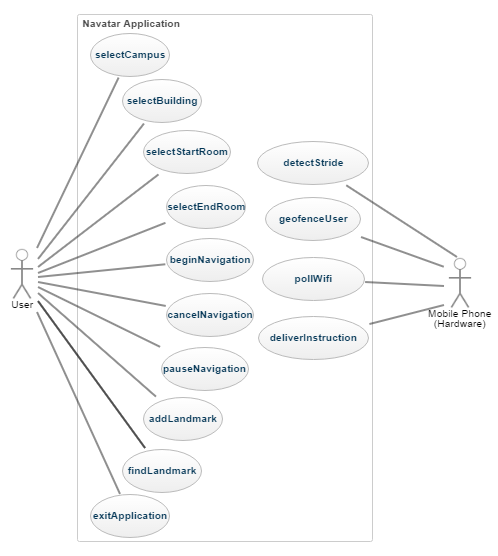
\includegraphics{ucd.png}

\begin{table}[ht]
	\section{Use Case Details}
\centering
\def\arraystretch{1.5}%
\resizebox{\textwidth}{!}{\begin{tabular}{| g | d | e |}
\hline
\rowcolor{LightCyan}
\mc{1}{Use Case Number}  & \mc{1}{Use Case Name} & \mc{1}{Description}\\
\hline
UC.01 & selectCampus     & The user selects a campus. This will then be the campus used for navigation.\\
\hline
UC.02 & selectBuilding   & The user selects a building. This will then be the building used for navigation. This can also be done with geofencing.\\
\hline
UC.03 & selectStartRoom  & The user selects a beginning point. The selected room is then used as the initial waypoint for navigation. \\
\hline
UC.04 & selectEndRoom    & The user selects a destination. The selected room is then used as the final waypoint for navigation. \\
\hline
UC.05 & beginNavigation  & The user begins navigating. Audio commands are delivered to the user to guide the user through an indoor environment.\\
\hline
UC.06 & cancelNavigation & The user opts to cancel navigation. If navigation is in progress, it is cancelled.\\
\hline
UC.07 & pauseNavigation  & The user chooses to pause navigation. If already paused, this resumes navigation.\\
\hline
UC.08 & addLandmark      & The user chooses to add a landmark. A screen allowing the user to add a landmark through gestures appears and the landmark is saved locally. Audio cues are also utilized for saving landmarks. \\
\hline
UC.09 & findLandmark     & The user searches for a saved landmark to use as a waypoint for navigation. This can be a starting or ending destination as well, or factored into an existing navigation path.\\
\hline
UC.10 & detectStride     & The hardware performs stride detection on the user as the user advances through the indoor environment. \\
\hline
UC.11 & geofenceUser     & The hardware uses geofencing to locate the building a user is in, specific to a selected campus.\\
\hline
UC.12 & pollWifi         & The hardware polls wifi SSID's for environmental information using the mobile phone's built-in wifi capabilities.\\
\hline
UC.13 & deliverInstruction  & The hardware delivers instructions through the audio port to the earbuds to guide the user. \\
\hline
\end{tabular}}
\end{table}

\begin{table}[ht]
\section{Use Case Templates}
\centering
\resizebox{0.8\textwidth}{!}{\begin{tabular}{| g | h | }
\hline
\rowcolor{LightCyan}
\mc{2}{\textbf{Use Case: geofenceUser}} \\
\hline
Use Case ID & UC.11\\ \hline
Actor & Hardware \\ \hline
Precondition(s) & 
\begin{enumerate}
	\item Application has been started.
	\item User's gps is enabled.
\end{enumerate} \\ \hline
Flow of Events & 
\begin{enumerate}
	\item Hardware uses gps to locate student using gps coordinate.
	\item Boundaries for the current campus are tested to see if the user is inside a building.
	\item If the user is found within the "geofence", the current building is automatically set.
\end{enumerate} \\ \hline
Postconditions(s) & 
\begin{enumerate}
	\item The current building is set.
	\item The current user's position is determined.
\end{enumerate} \\
\hline
\end{tabular}}

\centering
\resizebox{0.8\textwidth}{!}{\begin{tabular}{| g | h | }
\hline
\rowcolor{LightCyan}
\mc{2}{\textbf{Use Case: addLandmark}} \\
\hline
Use Case ID & UC.08\\ \hline
Actor & User \\ \hline
Precondition(s) & 
\begin{enumerate}
	\item The application has been started.
\end{enumerate} \\ \hline
Flow of Events & 
\begin{enumerate}
	\item The user chooses to add a landmark at the current position.
	\item An audio cue prompts the user for a name for the landmark.
	\item The user is prompted for saving the landmark.
	\item The landmark is saved.
\end{enumerate} \\ \hline
Postconditions(s) & 
\begin{enumerate}
	\item A landmark is added to the user's local landmarks for the current building and the current campus.
\end{enumerate} \\
\hline
\end{tabular}}

\centering
\resizebox{0.8\textwidth}{!}{\begin{tabular}{| g | h | }
\hline
\rowcolor{LightCyan}
\mc{2}{\textbf{Use Case: beginNavigation}} \\
\hline
Use Case ID & UC.05\\ \hline
Actor & User \\ \hline
Precondition(s) & 
\begin{enumerate}
	\item The application has been started.
	\item The user's gps is enabled.
\end{enumerate} \\ \hline
Flow of Events & 
\begin{enumerate}
	\item The user selects a start point in their geofenced building.
	\item The user selects an end destination for their geofenced building.
	\item The user is prompted for navigation.
	\item If approved, navigation is started.
\end{enumerate} \\ \hline
Postconditions(s) & 
\begin{enumerate}
	\item The software is in navigation mode.
	\item The user is being guided by the software through the indoor environment.
\end{enumerate} \\
\hline
\end{tabular}}
\end{table}

\chapter{Trace Matrix}
\begin{table}[h]
\centering
\caption{The trace matrix for Navatar's use cases and requirements.}
\label{my-label}
\resizebox{\textwidth}{!}{\begin{tabular}{|l|l|l|l|l|l|l|l|l|l|l|l|l|l|}
\hline
\rowcolor[HTML]{96FFFB} 
                             & UC.01                    & UC.02                    & UC.03                    & UC.04                    & UC.05                    & UC.06                    & UC.07                   & UC.08                    & UC.09                    & UC.10                    & UC.11                    & UC.12                    & UC.13                    \\ \hline
\cellcolor[HTML]{96FFFB}R.01 & {\color[HTML]{000000} }  & {\color[HTML]{000000} }  & {\color[HTML]{000000} }  & {\color[HTML]{000000} }  & {\color[HTML]{000000} X} & {\color[HTML]{000000} }  & {\color[HTML]{000000} } & {\color[HTML]{000000} }  & {\color[HTML]{000000} }  & {\color[HTML]{000000} }  & {\color[HTML]{000000} }  & {\color[HTML]{000000} }  & {\color[HTML]{000000} X} \\ \hline
\rowcolor[HTML]{C0C0C0} 
\cellcolor[HTML]{96FFFB}R.02 & {\color[HTML]{000000} }  & {\color[HTML]{000000} X} & {\color[HTML]{000000} X} & {\color[HTML]{000000} X} & {\color[HTML]{000000} X} & {\color[HTML]{000000} }  & {\color[HTML]{000000} } & {\color[HTML]{000000} }  & {\color[HTML]{000000} }  & {\color[HTML]{000000} }  & {\color[HTML]{000000} X} & {\color[HTML]{000000} }  & {\color[HTML]{000000} }  \\ \hline
\cellcolor[HTML]{96FFFB}R.03 & {\color[HTML]{000000} X} & {\color[HTML]{000000} }  & {\color[HTML]{000000} }  & {\color[HTML]{000000} }  & {\color[HTML]{000000} }  & {\color[HTML]{000000} X} & {\color[HTML]{000000} } & {\color[HTML]{000000} X} & {\color[HTML]{000000} }  & {\color[HTML]{000000} }  & {\color[HTML]{000000} }  & {\color[HTML]{000000} }  & {\color[HTML]{000000} }  \\ \hline
\rowcolor[HTML]{9B9B9B} 
\cellcolor[HTML]{96FFFB}R.04 & {\color[HTML]{000000} }  & {\color[HTML]{000000} }  & {\color[HTML]{000000} }  & {\color[HTML]{000000} }  & {\color[HTML]{000000} }  & {\color[HTML]{000000} }  & {\color[HTML]{000000} } & {\color[HTML]{000000} X} & {\color[HTML]{000000} X} & {\color[HTML]{000000} }  & {\color[HTML]{000000} }  & {\color[HTML]{000000} }  & {\color[HTML]{000000} }  \\ \hline
\cellcolor[HTML]{96FFFB}R.05 & {\color[HTML]{000000} }  & {\color[HTML]{000000} }  & {\color[HTML]{000000} }  & {\color[HTML]{000000} }  & {\color[HTML]{000000} }  & {\color[HTML]{000000} }  & {\color[HTML]{000000} } & {\color[HTML]{000000} X} & {\color[HTML]{000000} }  & {\color[HTML]{000000} X} & {\color[HTML]{000000} }  & {\color[HTML]{000000} X} & {\color[HTML]{000000} }  \\ \hline
\end{tabular}}
\end{table}

\chapter{Potential Legal Issues}

Navatar is free and open-source under the MIT license and hosted on GitHub.com. Because the software does not cost money, no software is being sold to users and thus no licenses are being infringed upon. Navatar and its creators assume no responsibility for any damages that occur during usage of the application. The software is safe and meant to be used as a software assistant. There are no potential legal issues under these circumstances that can be reasonably foreseen and accounted for at this time.

\begin{figure}[ht!]
\chapter{Snapshots}
\section{User Interface}
The screenshots below are mock-ups of what a visual user interface for this application might be. These screenshots demonstrate intended functionality that may actually be achieved through gestures on an otherwise empty screen in the application.
     \begin{center}
%
        \subfigure[Campus Selection]{%
            \label{fig:first}
            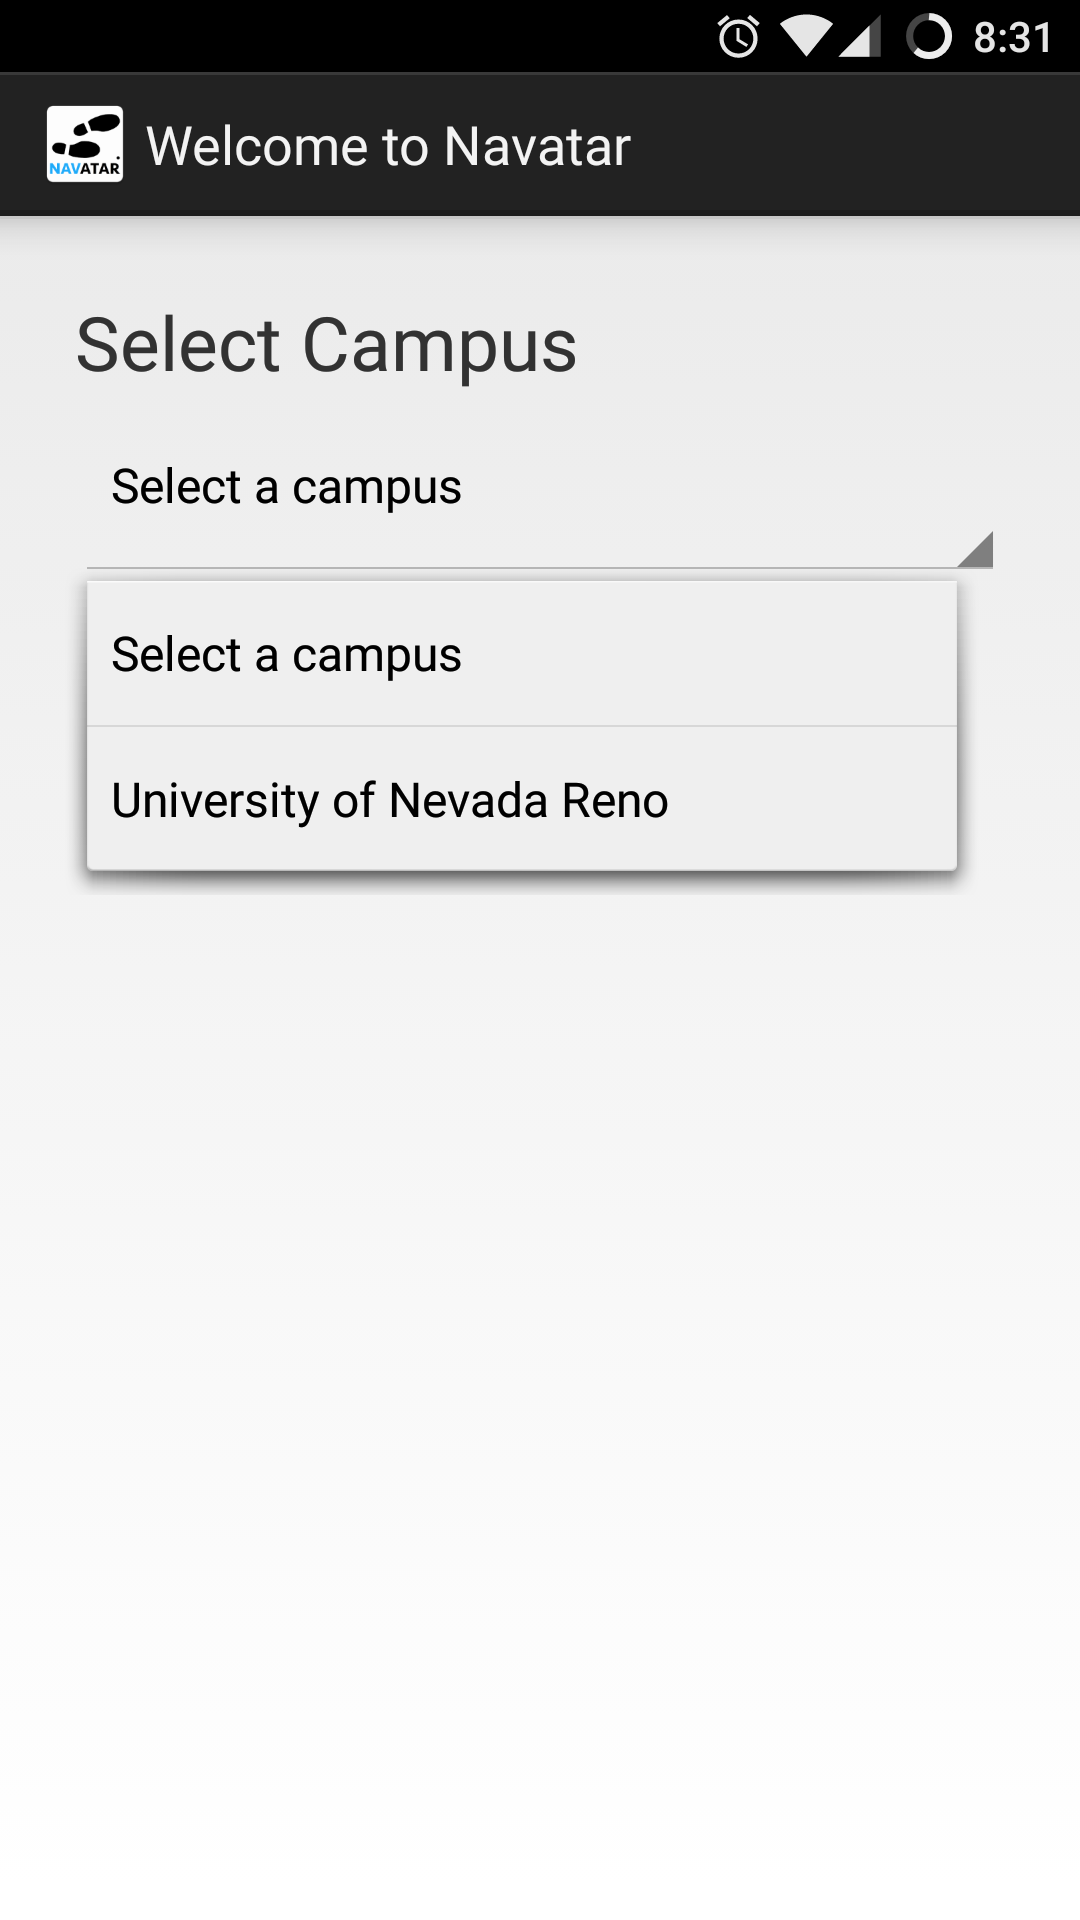
\includegraphics[width=0.3\textwidth]{1.png}
        }%
        \subfigure[Building Selection]{%
           \label{fig:second}
           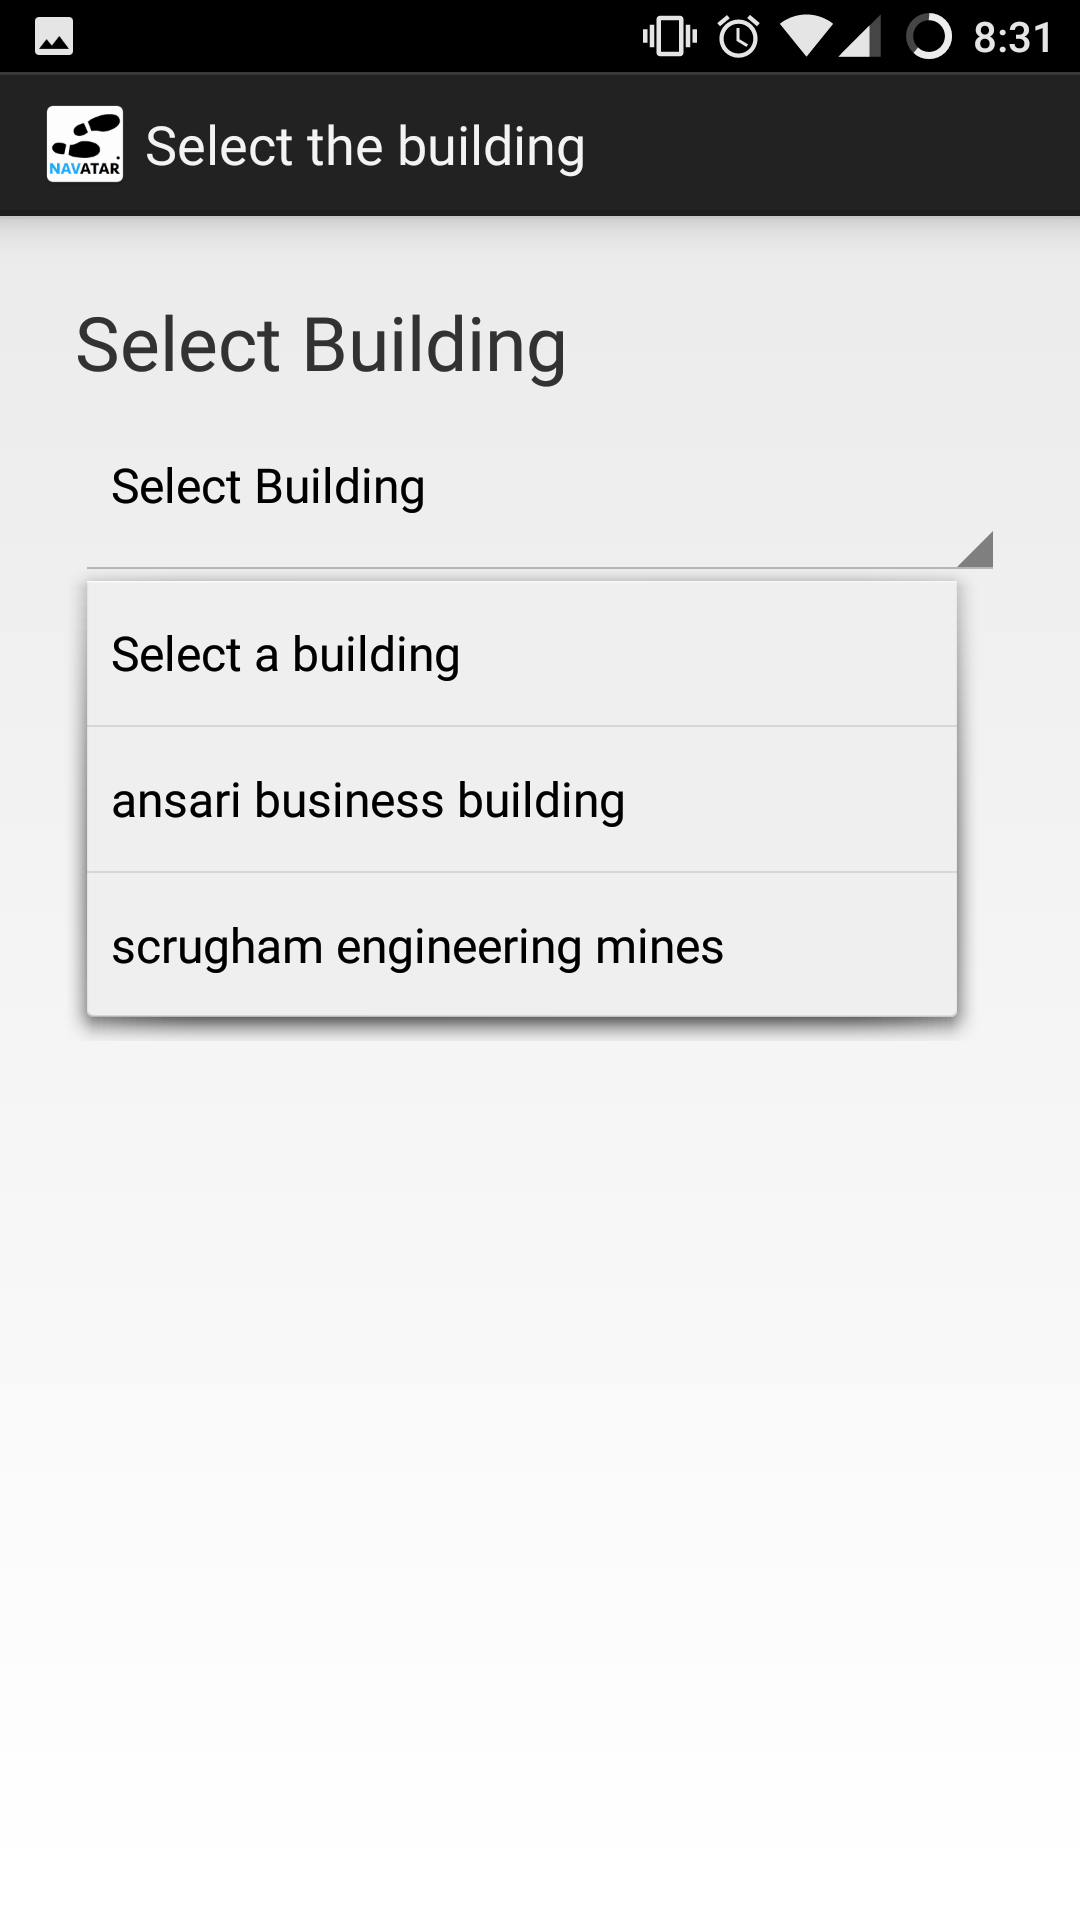
\includegraphics[width=0.3\textwidth]{2.png}
        } %  ------- End of the first row ----------------------%
        \subfigure[Starting Room Selection]{%
            \label{fig:third}
            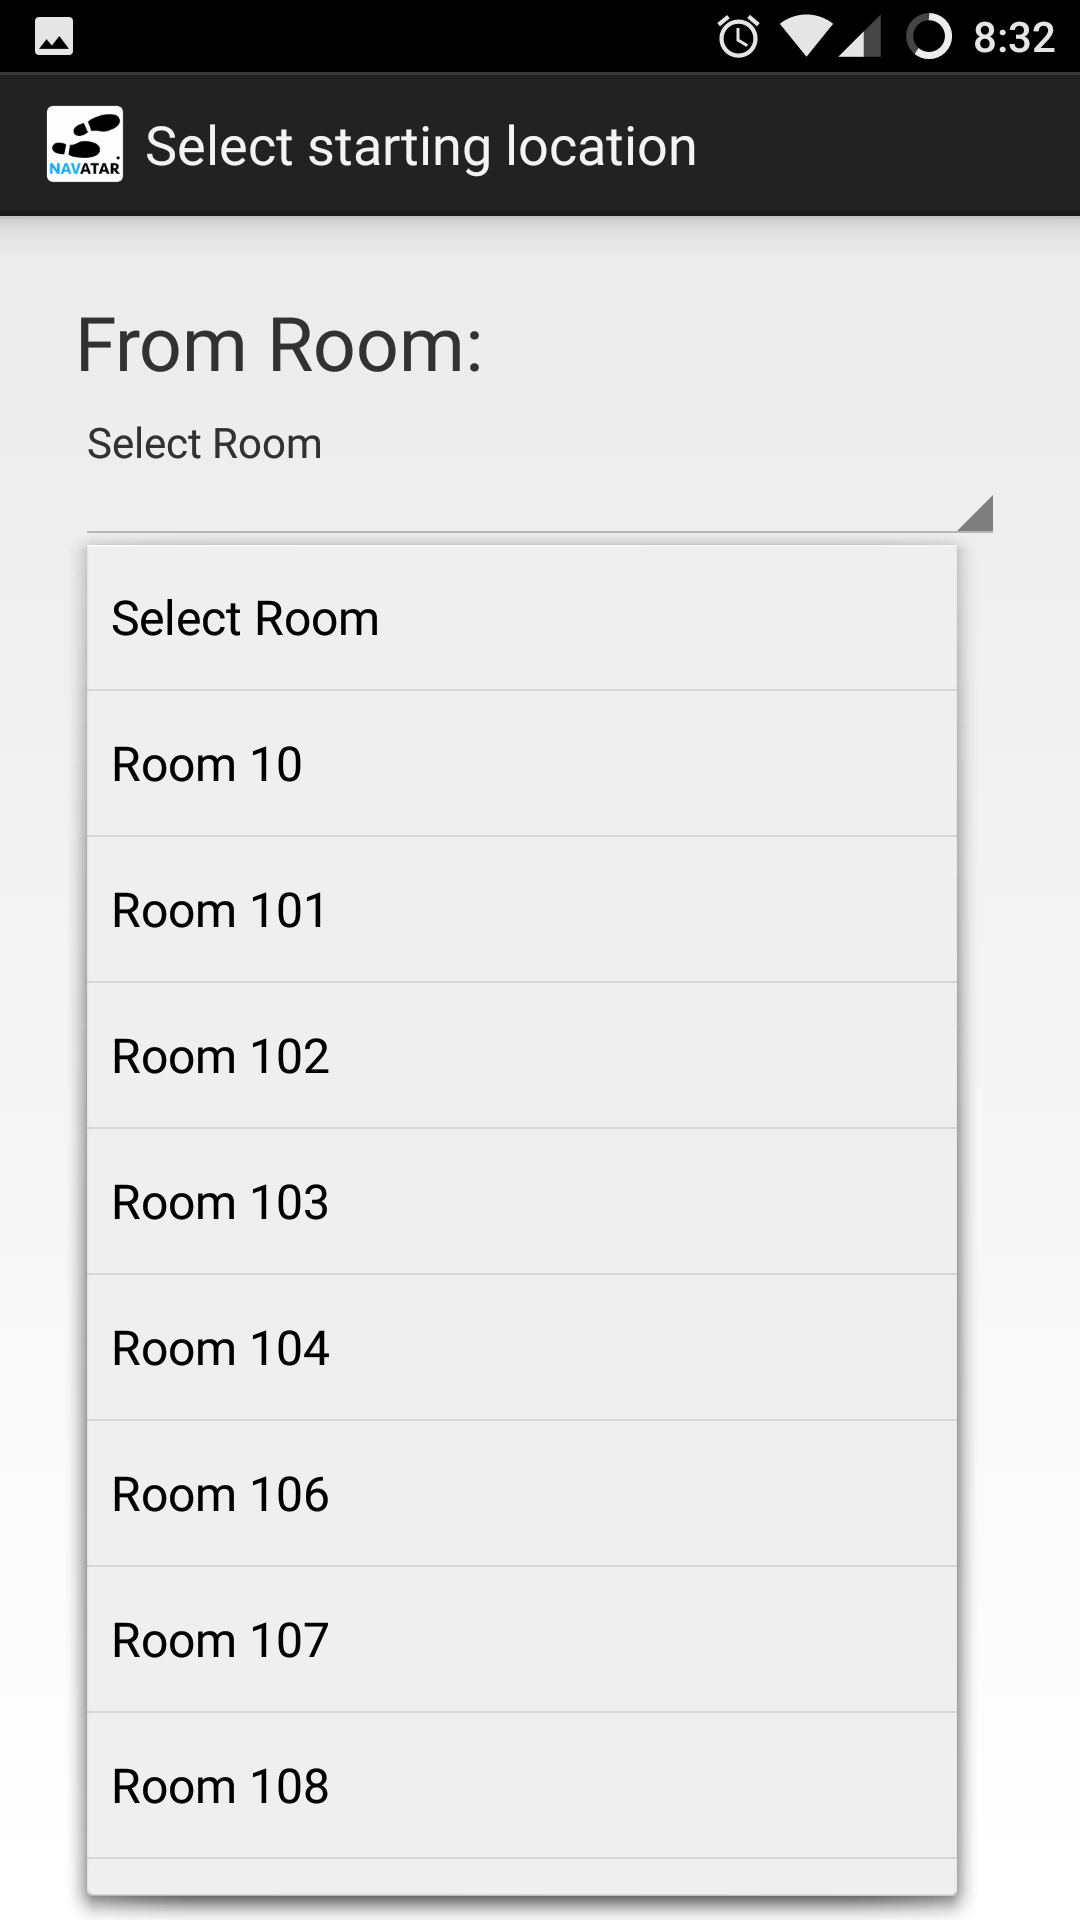
\includegraphics[width=0.3\textwidth]{3.png}
        }\\%
        \subfigure[Destination Room Selection]{%
            \label{fig:fourth}
            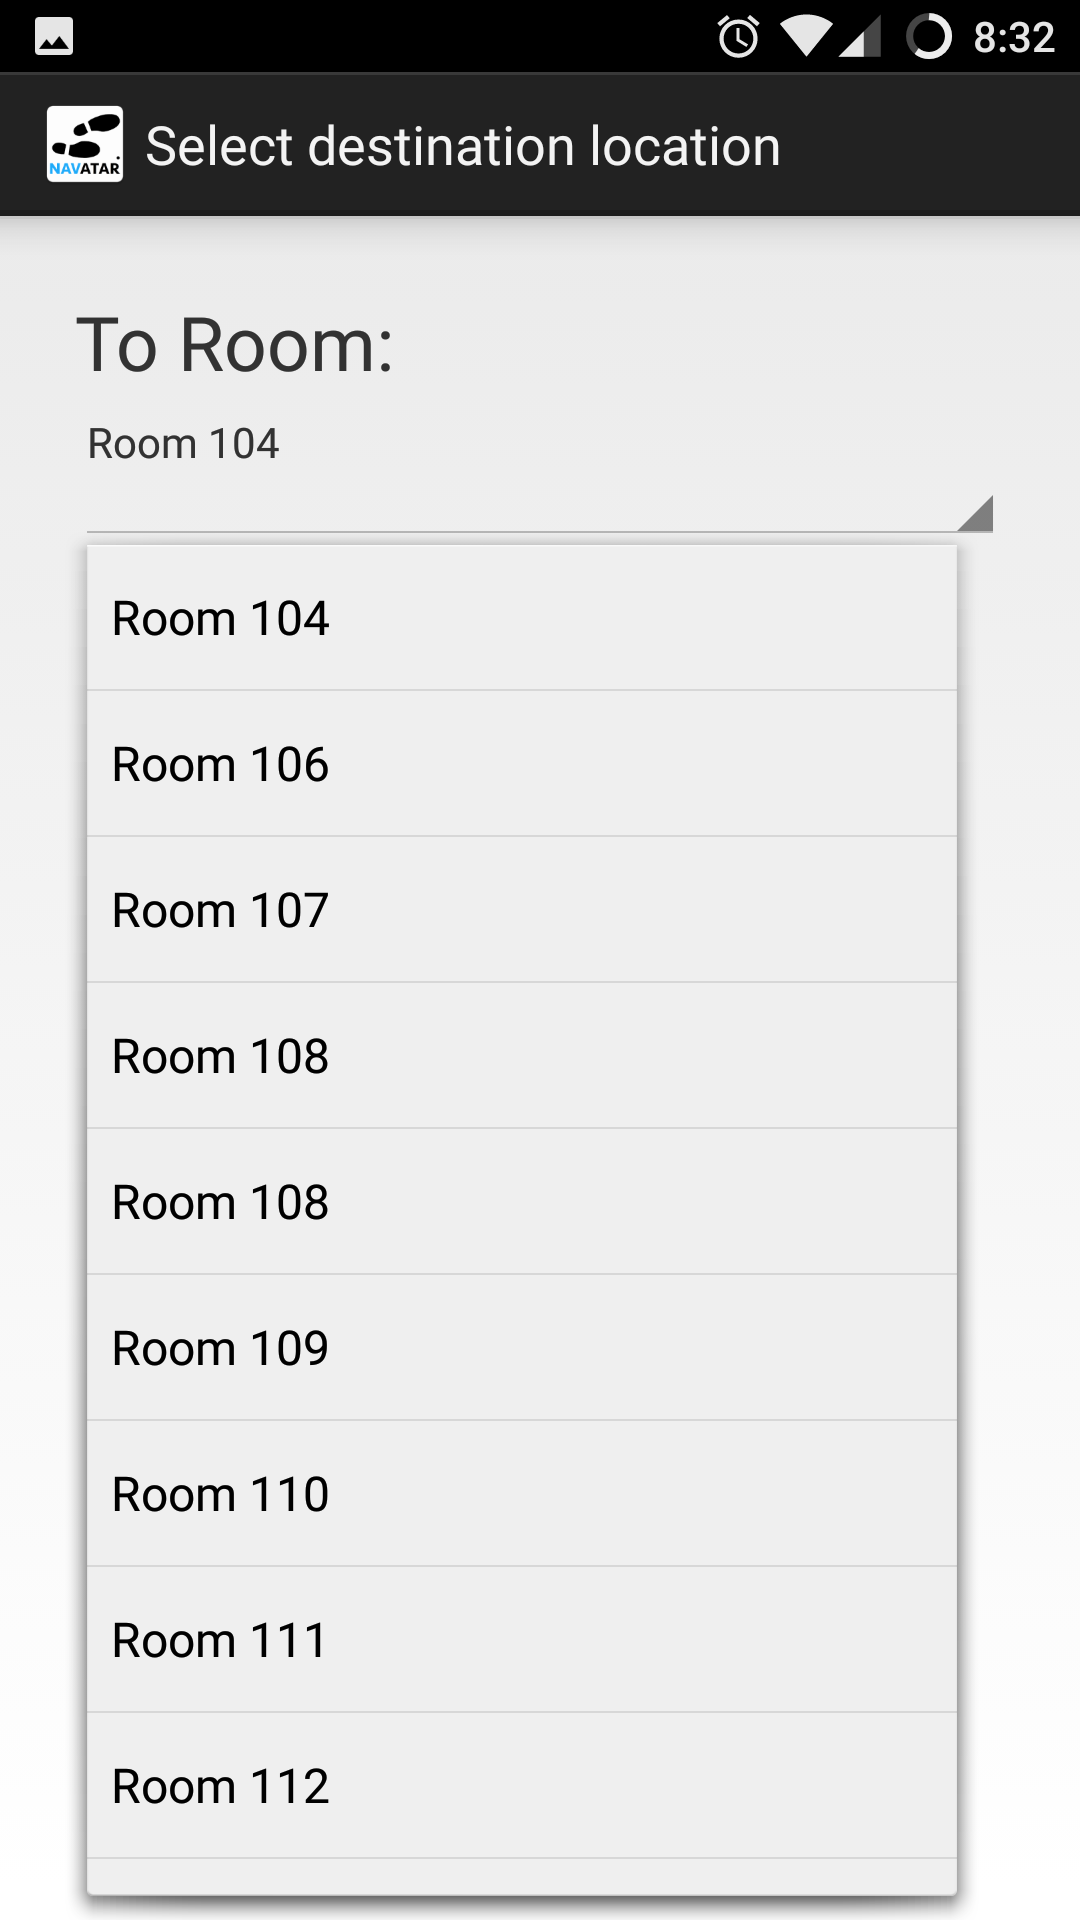
\includegraphics[width=0.3\textwidth]{4.png}
        }%
        \subfigure[Instruction Screen]{%
           \label{fig:fifth}
           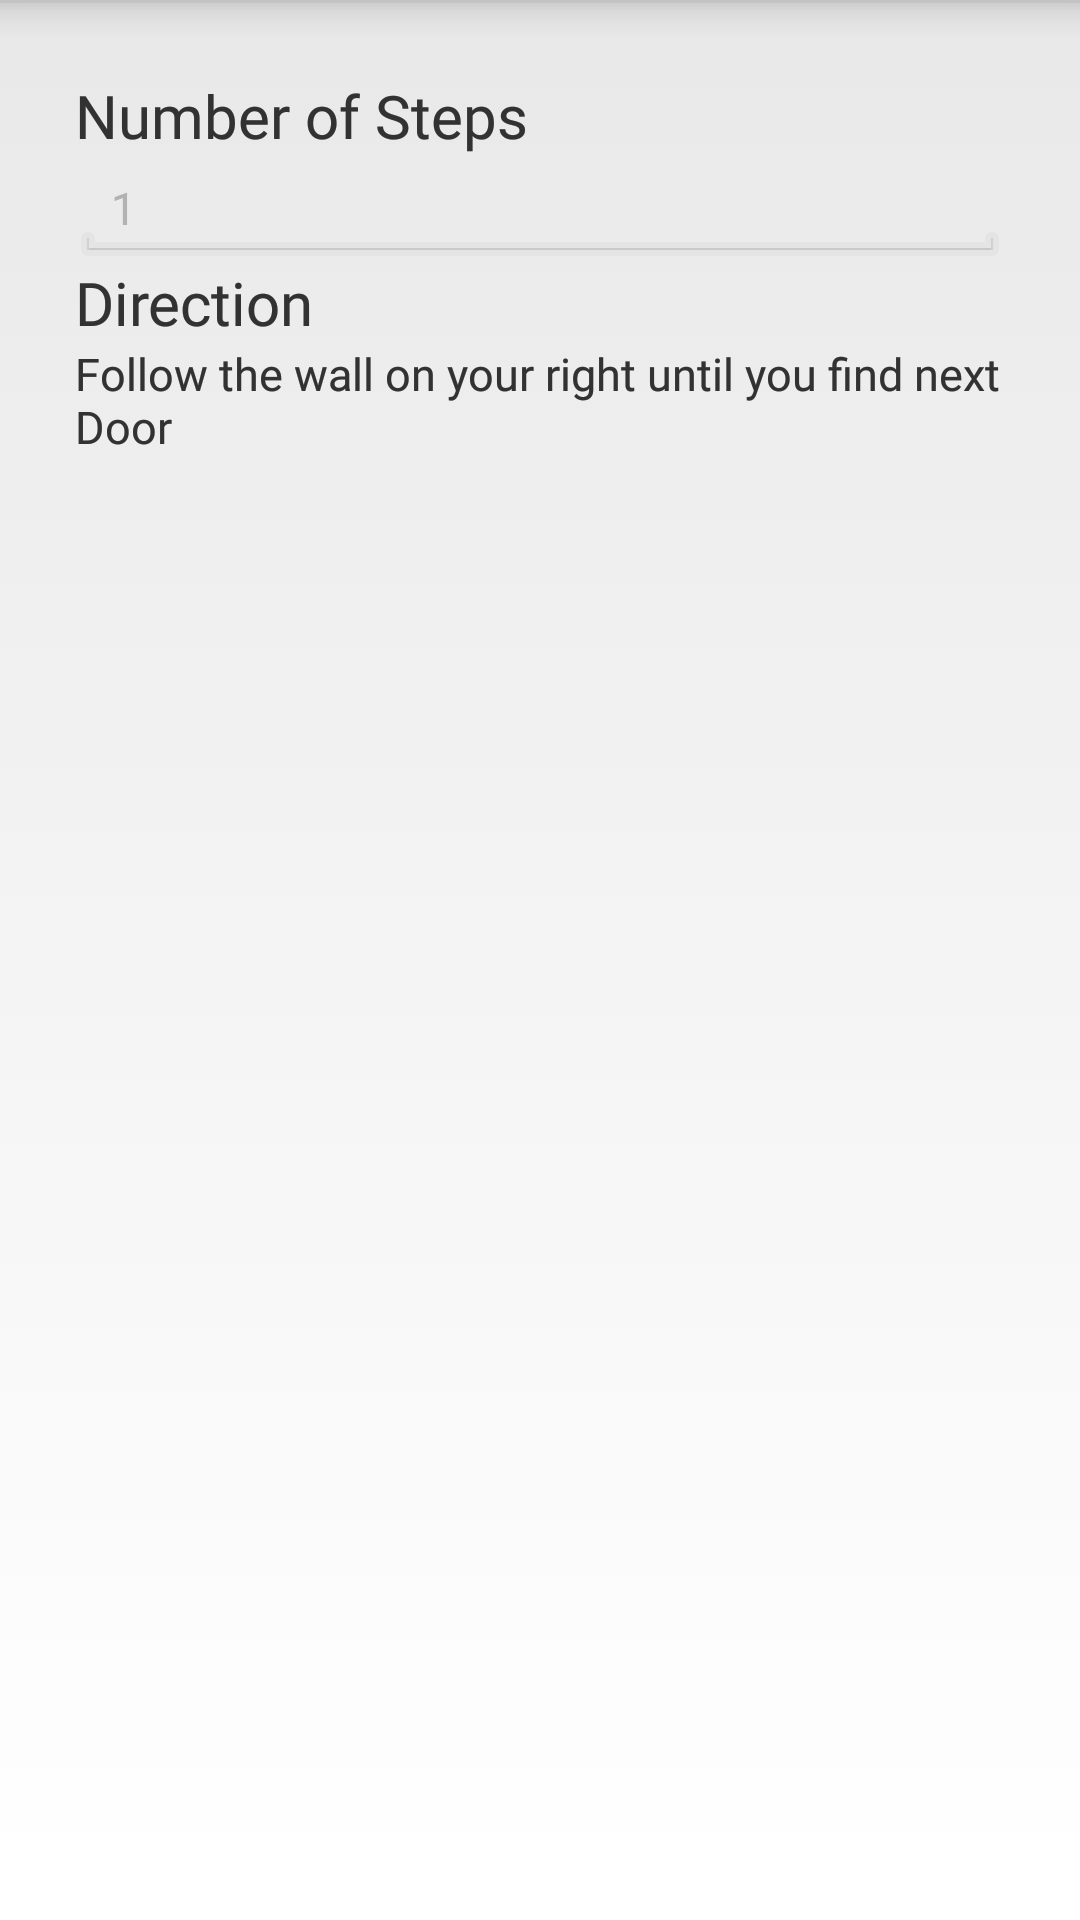
\includegraphics[width=0.3\textwidth]{5.png}
        } 
%
    \end{center}
    \caption{%
        Mock-up screenshots.
     }%
   \label{fig:subfigures}
\end{figure}

\begin{figure}[ht!]

\section{Layout}
     \begin{center}
%
        \subfigure[Home Screen]{%
            \label{fig:first}
            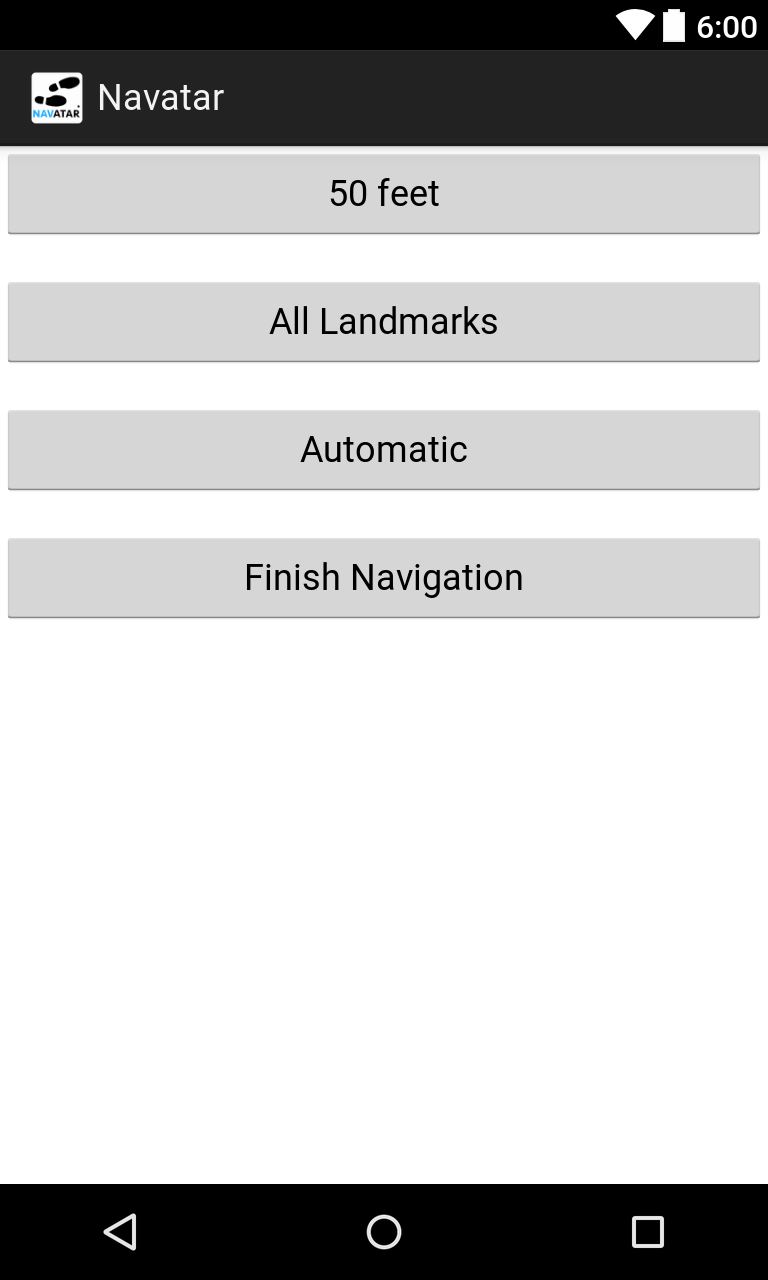
\includegraphics[width=0.3\textwidth]{11.png}
        }%
        \subfigure[Usage Selection]{%
           \label{fig:second}
           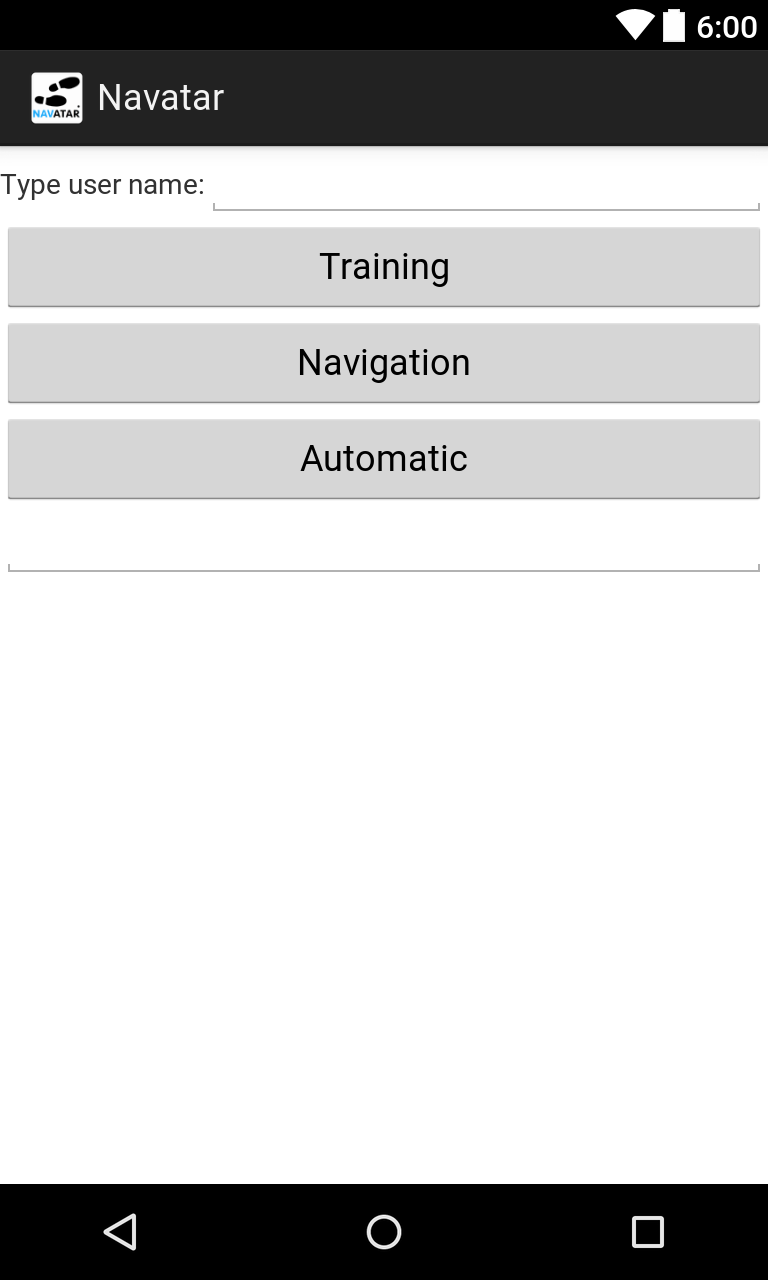
\includegraphics[width=0.3\textwidth]{12.png}
        } %  ------- End of the first row ----------------------%
        \subfigure[Campus Settings]{%
            \label{fig:third}
            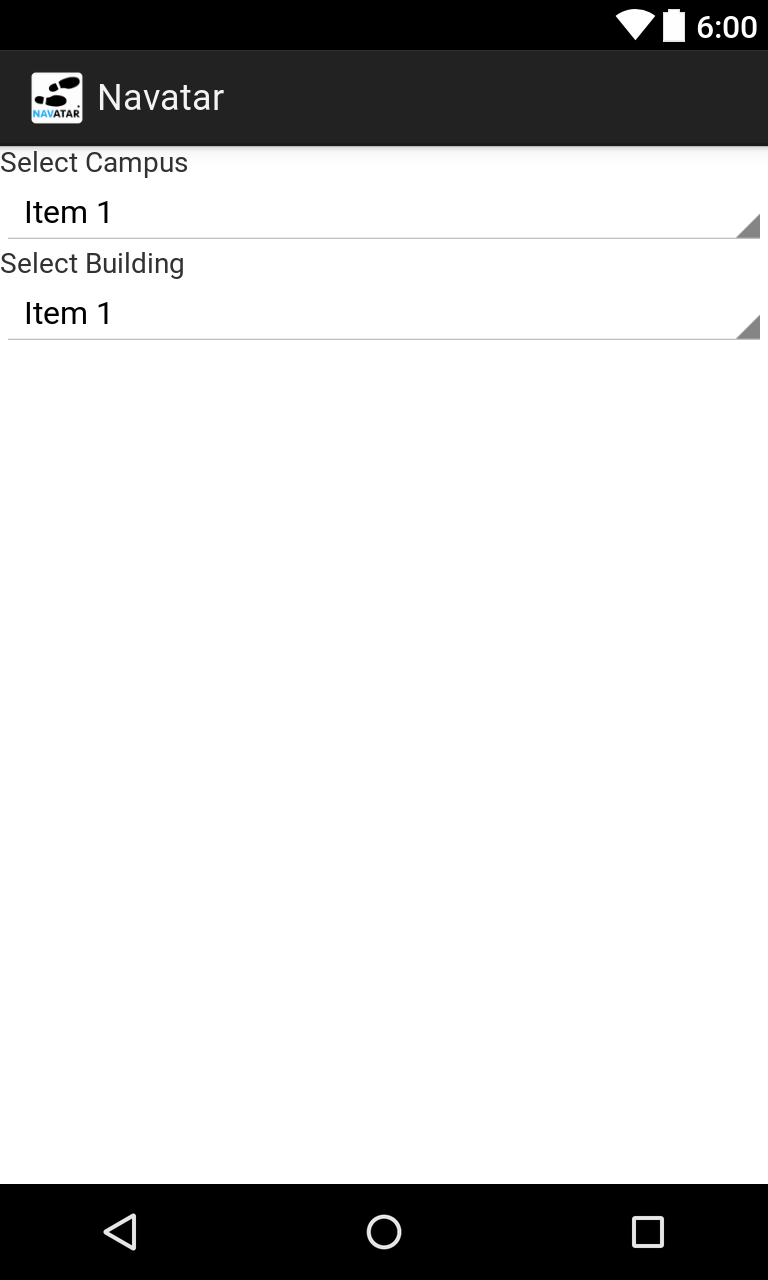
\includegraphics[width=0.3\textwidth]{13.png}
        }\\%
        \subfigure[Stride Settings]{%
            \label{fig:fourth}
            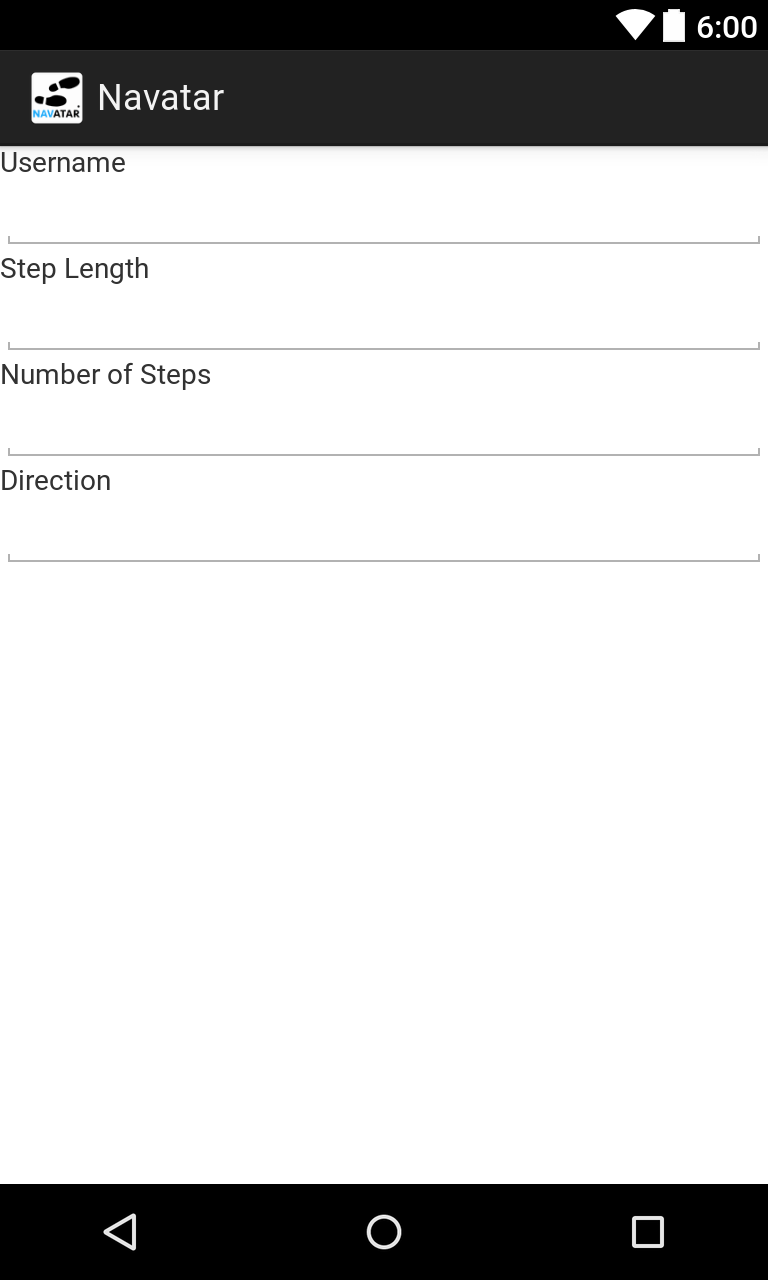
\includegraphics[width=0.3\textwidth]{14.png}
        }%
        \subfigure[Navigation Initialization]{%
           \label{fig:fifth}
           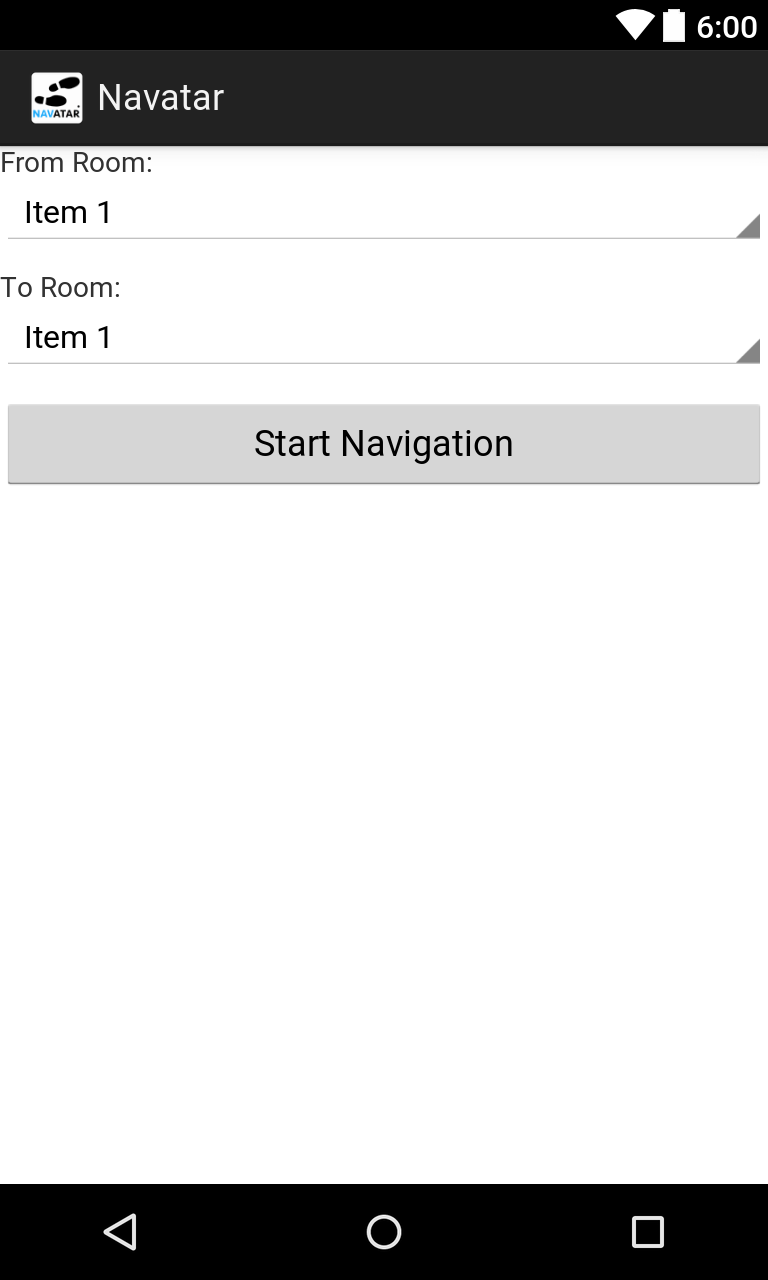
\includegraphics[width=0.3\textwidth]{15.png}
        } 
%
    \end{center}
    \caption{%
        Mock-up layouts of the interface.
     }%
   \label{fig:subfigures}
\end{figure}

\begin{table}[ht]
\chapter{Glossary}
\centering
\def\arraystretch{1.5}%
\resizebox{0.9\textwidth}{!}{\begin{tabular}{| a | b | }
\hline
\rowcolor{LightCyan}
\mc{1}{Term}  & \mc{1}{Definition} \\
\hline
Android & An operating system for mobile devices and smartphones. Navatar currently only supports this operating system.\\
\hline
 
Android Studio & An integrated development environment (IDE) for developing mobile applications for the Android operating system.\\
 
\hline
Dead-Reckoning & A localization technique that estimates a user’s location using an old estimated location as the starting point, using various data from sensors and other environment information to improve estimations.\\
 
\hline
Direct Sensing & A localization technique that uses physical identification tags to provide the current location of a user. Direct sensing requires the installation of these tags in the environment, which can be quite expensive.\\
 
\hline
Geofencing & Using global positioning systems to create geographical boundaries around an area, useful for determining what building a user of Navatar might be entering.\\
 
\hline
Geographic Information System (GIS) & a system used to store, manipulate, and present geographical data. Geographic information system maps are used by Navatar to load the layout of a given building.\\
 
\hline
Github & A web based service that hosts Git repositories to provide source control for software development purposes.\\

\hline
Global Positioning System (GPS) & A network of navigation satellites that provides geolocation information to a GPS receiver. GPS can be unreliable in indoor environments due to signal interference from the environment.\\

\hline
Landmark-based Navigation & Navigation using physical landmarks and a physical or mental map of the environment.\\

\hline
Localization & Adaptation of a product or service to meet the needs of a given language, culture, or population.\\
 
\hline
Pattern Recognition & Localization technique that uses previously stored environment data as a basis for determining a user’s location. A user then wears sensors that collects similar environment data which can be compared stored data to determine the user’s location.\\
 
\hline
Protobuffers or Protocol Buffers & A method of serializing, or converting data, to a storable format. Used by Navatar to store the GIS map data for buildings.\\
 
\hline
Radio Frequency Identifier Description (RFID) & Uses radio frequencies to uniquely identify an object or provide information about an object. RFID tags are used in some direct sensing localization systems to provide navigational information indoors.\\

\hline
Source Control & Also known as version control, is a system used to manage revisions to a software application's codebase. The history of all revisions is stored, allowing any previous revisions to be rolled back.\\

\hline
Stride detection & A method of determining a user's unique stride length and speed to improve location estimates.\\

\hline
\end{tabular}}
\end{table}

\chapter{References}

\section{Feasibility of Interactive Localization}
Ilias Apostolopoulos, Navid Fallah, Eelke Folmer, Kostas Bekris. Feasibility of Interactive Localization and Navigation of People with Visual Impairments, Proceedings of 11th Intelligent Autonomous Systems Conference, Pages 22-32, Ottawa, Ontario, August 2010.\\
 
 \textbf{Summary:}
 Investigates various solutions to the problem of indoor navigation for the visually impaired. Describes the issues that make indoor localization systems difficult to implement, and weighs the pros and cons of solutions that are currently available. Provides technical specifications for estimating a user’s location.
 
\section{Results from Initial User Experiments of Navatar}
Ilias Apostolopoulos, Navid Fallah, Eelke Folmer, Kostas Bekris, Integrated Online Localization and Navigation for People with Visual Impairments using Smart Phones, IEEE International Conference on Robotics and Automation (ICRA), Pages 1322 -1329, Minnesota, MN, May, 2012.\\

\textbf{Summary:}
Discusses the results from initial user experiments with the Navatar prototype, providing detailed statistical data and analysis. In depth description of Navatar’s path planning algorithm and accuracy. Shares some of the user’s experiences and feedback. Suggesting accuracy improvements, saving and repeating directions, and making the application hands free.

\section{Navatar’s Localization Architecture}
 Ilias Apostolopoulos, Navid Fallah, Eelke Folmer, Kostas Bekris. Integrated Online Localization and Navigation for People with Visual Impairments using Smart Phones, ACM Transactions on Interactive Intelligent Systems 3:4, Pages 1-25.\\

\textbf{Summary:}
More in depth descriptions of Navatar’s localization architecture, giving the actual algorithms used for sampling, as well as the transition and observation models. Shows how the K-Means algorithm can be used to adapt Navatar’s localization system to the unique stride lengths of a given user.

\section{Indoor Navigation System for the Blind}
Scientists design indoor navigation system for blind. (2016). Phys.org. Retrieved 8 November 2016, from http://phys.org/news/2012-05-scientists-indoor.html\\

\textbf{Summary:}
A high level overview of indoor localization systems, describing how Navatar uses a combination of GIS maps and readily available smartphone sensors to help visually impaired users navigate buildings. Contains some interview questions answered by Eelke Folmer about Navatar, and the potential benefits it could have.


\chapter{Contributions}
	\section{Matthew Berger}
		\begin{itemize}
			\item Created LaTeX document.
			\item Created Business requirements.
			\item Created Functional requirements.
			\item Created Non-Functional requirements.
		\end{itemize}
	\section{Connor Parkinson}
		\begin{itemize}
			\item Contacted blind students and conducted interviews.
			\item Created interview questions.
			\item Recorded interview answers and reviewed conversation logs.
			\item Provided detailed descriptions of accounts from potential-user interviews.
		\end{itemize}
	\section{Liam Gomez}
		\begin{itemize}
			\item Drafted user interface improvements.
			\item Drafted layout of components and took screenshots.
			\item Created a glossary with relevant terms.
			\item Provided articles and references, as well as summaries.
		\end{itemize}
\end{document}
